\documentclass[%
    paper=A4,               % paper size --> A4 is default in Germany
    twoside=true,           % onesite or twoside printing
    openright,              % doublepage cleaning ends up right side
    parskip=full,           % spacing value / method for paragraphs
    chapterprefix=true,     % prefix for chapter marks
    11pt,                   % font size
    headings=normal,        % size of headings
    bibliography=totoc,     % include bib in toc
    listof=totoc,           % include listof entries in toc
    titlepage=on,           % own page for each title page
    captions=tableabove,    % display table captions above the float env
    draft=false,            % value for draft version
]{scrreprt}

% !TEX root = my-thesis.tex


% **************************************************
% Files' Character Encoding
% **************************************************
\PassOptionsToPackage{utf8}{inputenc}
\usepackage{inputenc}
\usepackage[useregional]{datetime2}
\usepackage[german]{babel} % babel system, adjust the language of the content
\usepackage{amsmath}
\usepackage{listings}
\usepackage{pgfplots}
\usepackage{tabularx}
\usepackage{rotating}
\usepackage[toc,page]{appendix}

% **************************************************
% Information and Commands for Reuse
% **************************************************
\newcommand{\thesisTitle}{Optimierte Erstellung von Trainingsplänen für den Radsport}
\newcommand{\thesisName}{Jene-Julea Kabro}
\newcommand{\thesisSubject}{Bachelorarbeit}
\newcommand{\thesisSubmissionDate}{22. Februar 2020}
\newcommand{\thesisDate}{\thesisSubmissionDate}
\newcommand{\thesisVersion}{\today}

\newcommand{\thesisReviewer}{Dr. Stefan Endler}
\newcommand{\thesisReviewerUniversity}{\protect{\thesisUniversity}}
\newcommand{\thesisReviewerDepartment}{\thesisUniversityDepartment}

\newcommand{\thesisSupervisor}{Dr. Domenico Mosca}
\newcommand{\thesisSupervisorUniversity}{\protect{\thesisUniversity}}
\newcommand{\thesisSupervisorDepartment}{\thesisUniversityDepartment}

\newcommand{\thesisUniversity}{\protect{Johannes Gutenberg Universität Mainz}}
\newcommand{\thesisUniversityDepartment}{Fachbereich Physik, Mathematik und Informatik}
\newcommand{\thesisUniversityInstitute}{Institut für Informatik}
\newcommand{\thesisUniversityGroup}{Sportinformatik}
\newcommand{\thesisUniversityCity}{Mainz}
\newcommand{\thesisUniversityStreetAddress}{Saarstraße 21}
\newcommand{\thesisUniversityPostalCode}{55122}

% OWN COMMANDS
\newcommand*{\fullref}[1]{\hyperref[{#1}]{Kapitel \ref*{#1} -  \nameref*{#1}}} 

% **************************************************
% Debug LaTeX Information
% **************************************************
%\listfiles


% **************************************************
% Load and Configure Packages
% **************************************************
\PassOptionsToPackage{% setup clean thesis style
    figuresep=colon,%
    sansserif=false,%
    hangfigurecaption=false,%
    hangsection=true,%
    hangsubsection=true,%
    colorize=full,%
    colortheme=jgured,%
    bibsys=bibtex,%
    bibfile=bib-refs,%
    bibstyle=numeric,%
    wrapfooter=false,%
}{cleanthesis}


\usepackage{cleanthesis}

\hypersetup{% setup the hyperref-package options
    pdftitle={\thesisTitle},    %   - title (PDF meta)
    pdfsubject={\thesisSubject},%   - subject (PDF meta)
    pdfauthor={\thesisName},    %   - author (PDF meta)
    plainpages=false,           %   -
    colorlinks=false,           %   - colorize links?
    linkcolor=ctcolormain,      %   - link color (e.g., TOC)
    citecolor=ctcolormain,      %   - cite color
    pdfborder={0 0 0},          %   -
    breaklinks=true,            %   - allow line break inside links
    bookmarksnumbered=true,     %
    bookmarksopen=true          %
}

\begin{document}

% --------------------------
% rename document parts
% --------------------------
\renewcaptionname{german}{\figurename}{Abb.}
\renewcaptionname{german}{\tablename}{Tab.}

% --------------------------
% Front matter
% --------------------------
\pagenumbering{roman}			% roman page numbing (invisible for empty page style)
\pagestyle{empty}				% no header or footers
\begin{titlepage}
	\pdfbookmark[0]{Cover}{Cover}
	\flushright
	\hfill
	\vfill
	{\LARGE\thesisTitle \par}
	{\color{ctcolortitle}\rule[5pt]{\textwidth}{1pt} \par}
    % find das obere cooler
    % \rule[5pt]{\textwidth}{.4pt} \par
	{\Large\thesisName}
	\vfill
	\textit{\large\thesisDate} \\
	Version: \thesisVersion
\end{titlepage}


% ------------------------------------  --> main title page
\begin{titlepage}
	\pdfbookmark[0]{Titlepage}{Titlepage}
	\tgherosfont
	\centering

	{\Large \thesisUniversity} \\[4mm]
	
\includegraphics[width=6cm]{gfx/jgu_logo_quad.eps} \\[2mm]
	\textsf{\thesisUniversityDepartment} \\
	\textsf{\thesisUniversityInstitute} \\
	\textsf{\thesisUniversityGroup} \\

	\vfill
	{\large \thesisSubject} \\[5mm]
	{\LARGE \color{ctcolortitle}\textbf{\thesisTitle} \\[10mm]}
	{\Large \thesisName} \\

	\vfill
	\begin{minipage}[t]{.27\textwidth}
		\raggedleft
		\textit{Erstgutachter}
	\end{minipage}
	\hspace*{15pt}
	\begin{minipage}[t]{.65\textwidth}
		{\Large \thesisReviewer} \\
	  	{\small \thesisReviewerDepartment} \\[-1mm]
		{\small \thesisReviewerUniversity}
	\end{minipage} \\[5mm]
	
	\begin{minipage}[t]{.27\textwidth}
		\raggedleft
		\textit{Zweitgutachter}
	\end{minipage}
	\hspace*{15pt}
	\begin{minipage}[t]{.65\textwidth}
		{\Large \thesisSupervisor} \\
	    {\small \thesisSupervisorDepartment} \\[-1mm]
		{\small \thesisSupervisorUniversity}
	\end{minipage} \\[10mm]

	\thesisDate \\

\end{titlepage}


% ------------------------------------k+ü--> lower title back for single page layout
\hfill
\vfill
{
	\small
	\textbf{\thesisName} \\
	\textit{\thesisTitle} \\
	\thesisSubject\ vorgelegt am \thesisDate \\
	Erstgutachter: \thesisReviewer \\
	Zweitgutachter: \thesisSupervisor \\
	Betreuer: \thesisReviewer \\[1.5em]
	
	\textbf{\thesisUniversity} \\
	\textit{\thesisUniversityGroup} \\
	\thesisUniversityInstitute \\
	\thesisUniversityDepartment \\
	\thesisUniversityStreetAddress \\
	\thesisUniversityPostalCode\ \thesisUniversityCity
}
		% INCLUDE: all titlepages
\cleardoublepage

\pagestyle{plain}				% display just page numbers
\pdfbookmark[0]{Zusammenfassung}{Abstract}
\chapter*{Zusammenfassung}
\label{sec:abstract}
\vspace*{-10mm}
Besonders im Amateurbereich spielt die Vorbereitung zu den Wettkämpfen eine wichtige Rolle. Die maximale Leistung auf dem Rad wird vorallem von der physischen Leistungsfähigkeit beeinflusst. Unterschiedliche Trainingsziele nehmen Einfluss auf die Trainingsinhalte eines individuellen Sportlers. Mit personalisierten Trainingsplänen soll ein optimaler Trainingsverlauf für eine breite Personengruppe ermöglicht werden.
Um die Leistung zu steigern, wird diese Modellierung nach Erkenntnissen der allgemeinen und radsportspezifischen Trainingswissenschaft die Trainingseinheiten aufeinander abstimmen und so strukturieren, dass alle Leistungsbereiche wettkampfsorientiert gewichtet werden.
\vspace*{20mm}

{\usekomafont{chapter}Abstract}\label{sec:abstract-diff} \\
\vspace*{-10mm}
		% INCLUDE: the abstracts (english and german)
\cleardoublepage
%
\pdfbookmark[0]{Danksagung}{Danksagung}
\chapter*{Danksagung}
\label{sec:danksagung}
\vspace*{-10mm} % INCLUDE: acknowledgement
\cleardoublepage
%
\setcounter{tocdepth}{2}		% define depth of toc
\tableofcontents				% display table of contents
\cleardoublepage

% --------------------------
% Body matter
% --------------------------
\pagenumbering{arabic}			% arabic page numbering
\setcounter{page}{1}			% set page counter
\pagestyle{maincontentstyle} 	% fancy header and footer


\chapter{Einleitung}
\label{sec:einleitung}
\section{Motivation}
Im Amateursport sowie im Freizeitsport steht nur in seltenen Fällen eine persönliche Trainingsbetreuung zur Verfügung. Dennoch ist auch in diesem Bereich die Effektivität des Trainings abhängig von der Trainingsplanung. Neben der Optimierung der physiologischen Leistung bringt die Planung auch psychologische Vorteile mit sich \cite{ImplementationIntentions}. Die Vorgabe der Trainingszeiten kann zu einer höheren Verpflichtung und gesteigerten Motivation führen, sodass die geplanten Einheiten mit höherer Wahrscheinlichkeit umgesetzt werden.
Greift man auf vorgefertigte Trainingspläne zurück, büßt die Individualität des Trainingsplans ein. Die Qualität vorgefertigter Trainingspläne variiert stark je nach Quelle und ist ohne trainingswissenschaftliche Kenntnisse nicht zu beurteilen. Fehlen diese Kenntnisse, ist auch die eigene Anfertigung eines Trainingsplans zeitaufwändig. 
So entsteht ein Bedarf nach einer Modellierung auf Grundlage der radsportspezifischen Trainingswissenschaft, die die Erstellung eines individuellen Trainingsplans für Radsportlerinnen und Radsportler übernimmt. Personalisiert wird nach Trainingsziel und Einschränkungen im Trainingsumfang. 
Bereits bestehende Systeme sind nicht speziell für den Radsport entwickelt, haben keine individuelle Anpassung der Trainingseinheiten oder sind Teil von kostenintensiven Programmen.

\section{Problemstellung}
\label{sec:einleitung:problem}
Ziel der Arbeit ist die Entwicklung eines Programms zur automatisierten Erstellung von individuellen Trainingsplänen für Wettkampfdisziplinen im Radsport.
Das System modelliert auf Grundlage der allgemeinen und radsportspezifischen Trainingswissenschaften die Gestaltung der Trainingseinheiten einer drei- bis fünfmonatigen Aufbauperiode, die zyklisiert und periodisiert ist. Es ist möglich die Länge des Plans individuell zu wählen.
Typischerweise dient die Aufbauperiode zur Vorbereitung auf einen Wettkampf. Die physiologische Leistung wird vorwiegend durch die Abstimmung der Trainingseinheiten auf das Trainingsziel gesteigert. Im Straßenradsport betrifft das Trainingsziel den Bereich der Langzeitausdauer. Aus den unterschiedlichen Wettkampfarten kann dennoch eine Gewichtung der Belastungsbereiche geschlussfolgert werden. Entscheidend ist das Ziel also auch für ambitionierte Freizeitsportler, die anschließend keinen Wettkampf absolvieren.\par
Einen weiteren Einfluss auf die Trainingseinheiten hat der maximal verfügbare wöchentliche Trainingsumfang. Die verfügbaren Trainingstage und -stunden sind optimal zu nutzen, ohne sie zu überschreiten. 
Trotz der vielschichtigen Leistungsfaktoren eines erfolgreichen Wettkampfs behandelt der Plan ausschließlich die physische Leistungssteigerung. Andere Einflüsse auf die Leistung wie psychisches Belastungstraining, taktische Ausbildung, Ausrüstung oder Fahrbeschaffenheit \cite[13-15]{Radsporttraining} werden nicht im Rahmen dieser Arbeit behandelt.

\section{Zielgruppe}
Diese Modellierung richtet sich in erster Linie an den Amateursport und ambitionierten Freizeitsport, denn professionellen Sportler:innen steht im Normalfall Betreuungspersonal zur Verfügung. Bei der Fülle an Wettkämpfen in einer Saison wird in der Regel einem Wettkampf keine gesonderte Aufbauperiode gewidmet. Dieses System ist an Sportler:innen gerichtet, die ohne externe Betreuung trainieren. Für ambitionierte Freizeitsportler:innen, die im Anschluss an den Trainingsplan nicht an einem Wettkampf teilnehmen, kann dieser Plan für die Konzeption der Radsaison dienen. Dabei entspricht die Wettkampfdisziplin der Ausrichtung des Trainings.

\section{Überblick}
\label{sec:intro:ueberblick}
\textbf{\fullref{sec:verwandt}} \\[0.2em]
Ein Überblick über bereits bestehende Systeme und deren Eigenschaften. Verglichen wird nach den Kriterien Personalisierungsgrad, Komplexität und Funktionsumfang sowie den anfallenden Kosten für Benutzer:innen.

\textbf{\fullref{sec:grundlagen:rad}} \\[0.2em]
\hyperref[sec:grundlagen:rad]{Kapitel \ref{sec:grundlagen:rad}} befasst sich mit den Grundlagen der Sportwissenschaften sowohl im allgemeinen Bereich als auch den radsportspezifischen Anforderungen. Trainingseinheiten werden im Kontext der Periodisierung und Zyklisierung unterschiedliche Trainingsziele erfüllen und verschiedene Belastungsbereiche abdecken. Hier werden auch die verschiedenen Trainingsmethoden einer strukturierten Trainingseinheit vorgestellt.

\textbf{\fullref{sec:grundlagen:info}} \\[0.2em]
Die Modellierung erfolgt nach dem Programmierparadigma Constraint Programmierung. Dieses Verfahren verwendet Variablen und Constraints zur Beschreibung der Problemstellung. Ein Solver berechnet bei Existenz einer Lösung die Lösungsinstanz. 

\textbf{\fullref{sec:modellierung}} \\[0.2em]
Mit Hilfe der Grundlagen der Trainingswissenschaft wird der Trainingsplan modelliert. Die Anforderungen werden im Schema der Constraint Programmierung beschrieben. Zu Grunde liegt dabei ein mathematisches Modell, das die benötigten Variablen und Constraints definiert.

\textbf{\fullref{sec:implementierung}} \\[0.2em]
Vor der Implementierung des Modells mit Java wird das System konzipiert. Anhand von Klassendiagrammen visualisiert dieses Kapitel die Struktur der Implementierung. Vorrangig geht es um die Umsetzung der Modellierung und deren Einbindung in das objektorientierte Programm. Zusätzlich entsteht die grafische Schnittstelle für die Bedienung. Das Modell wird mit der Java-Bibliothek Choco Solver implementiert. Die Umsetzung ist als eigenständige Anwendung realisiert. 

\textbf{\fullref{sec:evaluation}} \\[0.2em]
Evaluiert wird ein dreimonatiger Trainingsplan, der aus der Anwendung erstellt worden ist. An dessen mittleren Umfang soll die Individualität der generierbaren Trainingspläne diskutiert werden. Thema ist auch die Performance des Lösungsprozesses.

\textbf{\fullref{sec:zusammenfassung}} \\[0.2em]
Abschließend wird ein Überblick von den Ergebnissen der Arbeit gegeben. Genauso beinhaltet dieses Kapitel den Ausblick über die möglichen Erweiterungen.
\chapter{Verwandte Arbeiten ?}
\label{sec:verwandt}
DIESES KAPITEL STREICHEN?

\section{Arbeit über Laufsport?}
\label{sec:verwandt:sec1}
\begin{itemize}
    \item andere Arbeit für laufsport?
    \item Kapitel sonst streichen
\end{itemize}
\chapter{Trainingswissenschaftliche Grundlagen}
\label{sec:grundlagen:rad}
Vor der Erstellung eines Modells gilt es die Merkmale eines optimalen Trainingsverlaufs zu spezifizieren. Dabei gibt es allgemeingültige sowie sportartspezifische Prinzipien der Gestaltung einer Trainingseinheit sowie darin enthaltener Trainingsabschnitte.

\section{Trainingsziel}
Macht man das Trainingsziel an einem Wettkampf fest, stellt sich immer die Frage nach der Wettkampfsdisziplin. Sportarten umfassen unterschiedliche Disziplinen, die jeweils andere Leistungsprofile erfordern. Im Radsport gibt es ein weites Spektrum von Wettkampfarten -- von weltbekannten Etappenrennen, wie der Tour de France bis hin zu Bahnradrennen. Diese beiden Beispiele gehen jedoch über die Zielgruppe dieser Arbeit hinaus, denn die Teilnehmenden erhalten professionelle Trainingsbetreuung wie im Profisport üblich. Im Amateursport sind dagegen folgende Wettkampfarten von größter Bedeutung.
\subsection{Eintagesrennen/Straßeneinzelrennen}
\label{eintagesrennen}
Das Eintagesrennen ist die älteste und verbreitetste Form der Straßenradrennen. Den ersten Platz erlangt die Person, die am schnellsten die Ziellinie erreicht.
Üblicherweise ist die Strecke geringer als 250 km. Die Belastung ist eng an das Streckenprofil (flach, wellig oder bergig) gekoppelt. So ist auch die Energiebereitstellung breit gefächert. Es wird sowohl auf den Fettstoffwechsel als auch auf den Kohlenhydratstoffwechsel zurückgegriffen. \TODO{Wichtig?} Das Training betrifft diverse Leistungsbereiche.
Ein ähnliches Belastungsprofil gilt beim Zeitfahren. Hier starten die Fahrer:innen jedoch einzeln und die gefahrenen Zeiten werden im Anschluss verglichen. Auf die Gewichtung der Leistungsbereiche hat dies jedoch keinen Einfluss. 
\subsection{Kriterium/Rundstreckenrennen}
Diese Disziplin unterscheidet sich von Eintagesrennen in der Länge der Strecke und der Art der Wertung. Eine Runde ist mit 800 Meter bis 10 Kilometer relativ kurz. Ein Rennen besteht aus mehreren Runden. 
Das beeinflusst maßgeblich das Leistungsprofil. \TODO{Hier genauer eingehen auf die Bereiche}
In die Wertung fließen Punktwertungen für Wertungssprints ein. 
\subsection{Bergzeitfahrt}
Wie in \ref{eintagesrennen} aufgegriffen, differenziert sich das Zeitfahren durch die Messung der Zeiten in aufeinanderfolgender Reihenfolge. Für die Definition der Leistungsbereiche entscheidend ist hier nur das Streckenprofil. Gesondert betrachtet wird also das Fahren am Berg, sogenannte Bergzeitfahrten. Das Training der Kraftausdauer ist hier von zentraler Rolle, um den Anstieg. \TODO{Auch hier genauer oder schöner formulieren}
\TODO{Zahlen anpassen!}
\begin{figure}[hb]
    \centering
        \begin{tikzpicture}
        \begin{axis}[
            xlabel={Leistungsbereiche},
            ylabel={Trainingsanteile (\%)},
            xmin=-0.5, xmax=5.5,
            ymin=0, ymax=100,
            xticklabels={KB, GA, EB, SB, K123, K45},
            ytick={0,20,40,60,80,100},
            xtick={0, 1, 2, 3, 4, 5},
            legend pos=north west,
            ymajorgrids=true,
            grid style=dashed,
        ]
        \legend{Straßeneinzel, Zeitfahrt, Bergfahrt}
        
        \addplot[ % Straßeneinzel
            color=red,
            mark=square,
            smooth
            ]
            coordinates {
            (0,5)(1,45)(2,15)(3, 10)(4, 10)(5,15)
            };
        \addplot[ % Zeitfahrt
            color=blue,
            mark=square,
            smooth
            ]
            coordinates {
            (0,10)(1,40)(2,15)(3,10)(4,10)(5,15)
            };
        \addplot[ % Bergfahrt
            color=green,
            mark=square,
            smooth
            ]
            coordinates {
            (0,0)(1,20)(2,20)(3,30)(4,10)(5,20)
            };
            
        \end{axis}
        \end{tikzpicture}
    \caption{Relevanz der Leistungsbereiche in verschiedenen Wettkampfsdisziplinen}
    \label{fig:wettkampfLeistungsbereiche}
\end{figure}

\section{Trainingsprinzipien}
\subsection{Periodisierung}
Zweck eines Trainingsplans ist es in einem Zeitrahmen individuelle Einheiten einzuplanen, um das persönliche Trainingsziel zu erreichen. Daraus hergeleitete Teilziele dienen einer detaillierteren Struktur. Die Granularität kann sogar bis zu einer individuellen Ausrichtung der Woche reichen. Jedes Teilziel wird in einer Periode behandelt, die Einfluss auf den Inhalt der Trainingseinheiten haben.\cite{periodization} \newline
Im Falle eines wettkampfsorientierten Trainingsjahres strebt man zum Wettkampf die maximale Leistungsfähigkeit an. Typischerweise setzt sich ein Trainingsjahr aus Vorbereitungsperiode, Aufbauperiode und Übergangsperiode zusammen.\cite[279]{Trainingswissenschaft} Die Vorbereitungsphase umfasst die Grundlagenausdauer und allgemeine Fitness. Im Radsport liegt diese im Allgemeinen in der Wintersaison. Innerhalb einer Aufbauperiode werden zunehmend die wettkampfsspezifischen Fähigkeiten ausgebaut. Das Training wird auf die individuellen Anforderungen eines Wettkampfs abgestimmt. Dabei kann abhängig von Länge und Anzahl der Wettkampfsphasen einfach oder mehrfach periodisiert werden.
\subsection{Zyklisierung}
Das Training gliedert sich in verschiedene Zyklen mit hierarchischem Aufbau. Sie geben dabei die Belastung und Regenerationsphasen im Trainingsplan vor. Übergeordnete Stufen wirken auf darunterliegende Zyklen ein, indem sie Trainingsumfang, Methoden und auch die Wahl der Leistungsbereiche beeinflussen. \cite[283]{Trainingswissenschaft}
Makrozyklen haben eine Dauer von 4-5 Monaten. Sie bestehen aus Mesozyklen, die eine Dauer von circa 4 Wochen haben. Jede Woche wird dabei als Mikrozyklus bezeichnet. Darin werden Trainingseinheiten geplant. Sogenannte strukturierte Trainingseinheiten definieren zusätzlich die enthaltenen Trainingsabschnitte. Maßgeblich für die Unterteilung einer Einheit ist dabei die Trainingsmethode aus dem Kapitel \ref{grundlagen:methoden}.
\subsection{progressive Belastungssteigerung}
Nach einem Trainingsreiz über der Reizschwelle reagiert der Körper mit Anpassungen. Die Leistung wird gesteigert, indem die Reizschwelle erhöht wird. Weitere Leistungssteigerungen durch Anpassungen des Körpers treten erst ein, wenn die veränderte Reizschwelle übertroffen wird. Die Belastung durch Trainingseinheiten erzielt eine optimale Leistungssteigerung, wenn sie progressiv gestaltet ist. Jedoch schädigt ein zu starker überschwelliger Reiz das System. Bei unterschwelligen Reizen führen die Trainingseinheiten nicht zur Steigerung der Leistung, da keine körperliche Anpassung stattfindet. \cite[58]{Seidenspinner2005} Progression kann dabei durch Steigerung der wöchentlichen Trainingstage, der Dauer der Einheiten oder der Trainingsintensität erreicht werden. Möglich ist auch die Verkürzung der Pausen.\newline 
Mesozyklen und Makrozyklen sind je mit steigender Belastung geplant. Der Trainingsumfang dient hier als Richtwert. \cite[60-61]{Radsporttraining}
\subsection{Regeneration}
Die Anpassung des Körpers an neue überschwellige Reize erfolgt nicht beim Training selbst, sondern in der Regenerationszeit. Um Übertraining zu verhindern, ist mindestens ein Regenerationstag in der Woche einzuplanen. 
Zur optimalen Leistungssteigerung werden sowohl Trainingseinheiten als auch Belastungspausen zwischen den Einheiten eingeplant. Die Länge der Regenerationspause ist dabei abhängig von Intensität und Dauer der vorangegangenen Leistung. Auch Alter, Geschlecht, Ernährung oder Tagesform spielen eine Rolle. Trotzdem verlieren einige Richtlinien nicht die Allgemeingültigkeit. Beispielsweise folgt nach Wettkämpfen immer eine Phase der Regeneration. Diese kann auch als aktive Regeneration gestaltet sein. Das sind Trainingseinheiten mit geringster Intensität.
\subsection{Superkompensationsmethode}
Die Superkompensation bezeichnet die gesteigerte Leistungsfähigkeit bei optimaler Zeitplanung der Regeneration nach einer Belastung.\cite[163]{Trainingswissenschaft} Dabei ist Übertraining aber auch Unterforderung zu vermeiden um eine bestmögliche Belastung zu erreichen. In der Erholungsphase gibt es einen Zeitpunkt, an dem erhöhte Leistungsbereitschaft besteht. Der Zeitpunkt ist abhängig von Intensität und Umfang der jeweiligen Einheit aber auch von persönlichen Voraussetzungen wie Leistungsstand und Erholungsfähigkeit. \newline
Folgende Richtlinien ergeben sich für die Trainingsplanung. \cite[44-46]{Radsporttraining} Nur eine Trainingseinheit pro Tag wird eingeplant bei mehrstündigen Ausdauerbelastungen. Die Belastung sollte dabei im Block erfolgen -- circa drei bis fünf aufeinanderfolgende Tage bei Einheiten für die Grundlagenausdauer. Bei Einheiten mit hoher Intensität sind die Blöcke kürzer gestaltet. Im Anschluss an einen Belastungsblock folgt ein Regenerationstag. An Erholungstagen ist keine Trainingseinheit oder maximal eine Belastung im Regenerationsbereich erlaubt. Einheiten im Bereich des Krafttrainings werden bevorzugt nach einem Regenerationstag eingeplant. 
\TODO{Nicht benutzt? \cite[60]{Radsporttraining}}

% \section{Trainingseinheit}
%\label{grundlagen:einheiten}
%Sind Trainingspläne monoton gestaltet, kann es zu Übertraining, Leistungsstagnation oder Krankheit kommen. Diese werden unterbunden durch strukturierte Trainingseinheiten, die in verschiedene Trainingsabschnitte geteilt werden. Dabei variieren die Einheiten in der Trainingsmethode und den enthaltenen Leistungsbereichen.
\section{Belastungsbereiche}
\label{grundlagen:sport:belastungsbereiche}
Die Aufbauphase dient zur Vorbereitung auf einen Wettkampf. Im Radsport gibt es verschiedene Disziplinen (Straßenrennen, Zeitfahrten, Bergfahrten, uvm.) mit unterschiedlichem Belastungsprofil. Um die wettkampfsspezifischen Anforderungen zu trainieren, werden die Leistungsbereiche des Radsports in dessen Abhängigkeit gewichtet. \TODO{ergibt der Satz Sinn?} Maßgeblich ist die Intensität der Belastung. Folgende Einteilung der Bereiche findet man in Lindners Radsporttraining. \cite[31-39]{Radsporttraining} Obwohl die Benennung nicht übereinstimmt, wurde in vergleichbarer Literatur \cite[27]{Ausdauertrainer} eine analoge Einteilung in sieben Stufen vorgenommen.
\subsection{Kompensationsbereich (KB)}
Der Leistungsbereich mit niedrigster Intensität ist der Kompensationsbereich. Dieses Training belastet mit 60\% der maximalen Herzfrequenz. Es wird eingesetzt zur aktiven Regeneration oder Kompensation. Üblicherweise folgt ein Kompensationstraining nach sehr intensiven Einheiten oder Wettkampfsbelastungen. Beispiele für ein Kompensationstraining sind Ausfahrten oder Läufe mit geringer Intensität, Spaziergänge oder Mobilisationstrainings. \cite[31-32]{Radsporttraining}
Eine Regenerationsfahrt hat eine maximale Länge von 2 Stunden. Das alternative Lauftraining sollte 45 Minuten nicht übersteigen und ist nur außerhalb der Rennsaison empfohlen.
\subsection{Grundlagenausdauer (GA)}
Trainingseinheiten mit leichter Intensität werden für die Entwicklung der Grundlagenausdauer verwendet. Sie steigern die Leistung im aeroben Bereich \TODO{Definition} und trainieren so denn Fettstoffwechsel.
Training im Grundlagenausdauerbereich ist auch für die Einheiten mit hoher Intensität von Bedeutung. Die Grundlagenausdauer nimmt einen großen Teil des Trainingsplans ein.
\subsection{Entwicklungsbereich (EB)}
Im Entwicklungbereich wird die wettkampfsspezifische Ausdauer im mittleren Intensitätsbereich trainiert. Zusätzlich zum Fettstoffwechsel bindet es auch den Kohlenhydratstoffwechsel ein. Es wird im aeroben-anaeroben Bereich traininert. Oft wird es als Wiederholungsmethode durchgeführt.
\subsection{Spitzenbereich (SB)}
Die hohe Intensität im Spitzenbereich verwendet den Kohlenhydratstoffwechel. Hier wird die anaerobe Schwelle übertroffen. Ziel ist es die Schnelligkeit und Schnelligkeitsausdauer auf die Wettkampfsbedingungen zu entwickeln. Überwiegend sind Trainingseinheiten mit der Intervallmethode strukturiert und unmittelbar vor Wettkämpfen platziert.
\subsection{Maximal- und Schnellkraftsbereich (K1-K2)}
Im aeroben Bereich befindet sich die Entwicklung der Maximal- und Schnellkraft. Besonders bei Strecken mit hoher Steigung und Bergfahrten gewinnt dieser Bereich an Bedeutung. Die Maximal- und Schnellkraft ermöglicht es hohe Übersetzungen auch mit hoher Tretfrequenz zu beherrschen. Häufig wird dafür die Wiederholungsmethode eingesetzt.
\subsection{Kraftausdauer (K3-K4-K5)}
Auch hier ist das Trainingsziel eine hohe Tretfrequenz mit hoher Übersetzung zu fahren. Diese soll auch über längere Zeit gehalten werden. Die Energiebereitstellung ist im aerob-anaeroben Übergangsbereich. Bergfahrten mit Tempo- und Rythmuswechsel sind eine mögliche Trainingseinheit für diesen Leistungsbereich.

\section{Trainingsmethoden}
\label{grundlagen:methoden}
\newcolumntype{b}{>{\hsize=0.4\hsize}X}
\newcolumntype{s}{>{\hsize=0.1\hsize}X}

Der Aufbau einer Trainingseinheit wird durch die Trainingsmethode bestimmt. Im Folgenden handelt es sich lediglich um eine Auswahl der möglichen Trainingsmethoden für Radsportler:innen in der Aufbauphase.  \cite[40-43]{Radsporttraining} \TODO{reicht es hier zu zitieren?}
\subsection{Dauerleistungsmethode DL}
Bei der Dauerleistungsmethode wird die gesamte Trainingseinheit in einem Leistungsbereich ausgeführt. Oft findet diese in niedrigeren Intensitäten Verwendung. Ein Großteil der Vorbereitungsphase priorisiert das Training des Grundlagenausdauerbereichs, der mit der Dauerleistungsmethode trainiert wird.
Das Training dreht sich um einen einzelnen Leistungsbreich, aber Einheiten mit hoher Intensität erfordern kurze Aufwärm- und Ausfahrzeiten im Grundlagenausdauerbereich.
\begin{table}[h]
\centering  
    \begin{tabularx}{\textwidth}{|b|ssssss|}
    \hline
    \textbf{Einheit} & \textbf{KB} & \textbf{GA}& \textbf{EB}& \textbf{SB}& \textbf{K123}   &\textbf{K45} \\  \hline
    Kompensationsfahrt                  & 30-120 &         &             &        &        &           \\ \hline
    Extensive Fahrt                     &        & 60-240  &             &        &        &           \\ \hline
    Fettstoffwechselfahrt               &        & 180-360 &             &        &        &           \\ \hline
    Intensive Fahrt                     &        & 60      & 15-60       &        &        &           \\ \hline
    Extensive Kraftausdauer Fahrt       &        & 30-60   &             &        & 30-150 &           \\ \hline
    Einzelzeitfahrt                     &        & 60      &             & 30-60  &        &           \\ \hline
    \end{tabularx}
    \caption{Trainingseinheiten mit der Dauerleistungsmethode}
    \label{table:fahrtspiel}
\end{table}
\subsection{Fahrtspiel FS}
Das Fahrtspiel ist eine spezielle Art der Dauerleistungsmethode. Dabei gibt es keine Vorgaben hinsichtlich der Intensität und des Leistungsbereichs. Die Belastung erfolgt ohne Pause, kann aber mehrere Leistungsbereiche ansprechen. Das Training wird persönlich gesteuert oder kann durch die äußeren Gegebenheiten (bergiger Streckenverlauf) beeinflusst werden. Vorgaben über Anteile der Trainingsbereiche sind zeitlich flexibel eingebaut. Nicht jeder Leistungsbereich muss dabei abgedeckt werden. 

\begin{table}[h]
\centering  
    \begin{tabularx}{\textwidth}{|b|ssssss|}
    \hline
    \textbf{Einheit}                     & \textbf{KB}     & \textbf{GA}      & \textbf{EB}          & \textbf{SB}     & \textbf{K123}   & \textbf{K45}       \\    \hline
    Extensives Fahrtspiel               &       & 60-240    & 60-240    &           &       &       \\\hline
    Intensives Fahrtspiel               &       & 60-180    & 60-180    & 60-180    &       &       \\\hline
    \end{tabularx}
    \caption{Trainingseinheiten mit der Fahrtspielmethode}
    \label{table:fahrtspiel}
\end{table}

\subsection{Intervallmethode IV}
Intervalleinheiten alternieren Belastung und Erholungsphasen. Die Pausen reichen nicht für eine vollständige Erholung aus und können auch als aktive Pausen gestaltet werden. Bei aktiven Pausen wird das Training nicht vollständig unterbrochen, sondern mit geringer Aktivität weitergeführt. Serienpausen sind längere Pausen und gruppieren mehrere Belastungen. Besonders Einheiten mit hoher Intensität werden mithilfe der Intervallmethode trainiert. 
\begin{table}[h]
\centering
    \begin{tabularx}{\textwidth}{|b|ssssss|}
    \hline
    \textbf{Einheit}                     & \textbf{KB}     & \textbf{GA}      & \textbf{EB}          & \textbf{SB}     & \textbf{K123}   & \textbf{K45}       \\    \hline
    Intensive Kraftausdauer Fahrt (Berg) &        & 30-90   &             &        &        & 15-120  \\\hline
    Schnelligkeitsausdauer               &        & 60-180  &             & 15-45  &        &           \\ \hline               
    \end{tabularx}
    \caption{Trainingseinheiten mit der Intervallmethode}
    \label{table:intervallmethode}
\end{table}

\subsection{Wiederholungsmethode WH}
Ähnlich wie in der Intervallmethode gibt es einen Wechsel zwischen Belastung und Erholung. Jedoch dienen die Pausen bei der Wiederholungsmethode der vollständigen Erholung. Anhand der Herzfrequenz kann kontrolliert werden, zu welchem Zeitpunkt die nächste Belastung startet. Auch hiermit werden tendenziell Trainingsbereiche mit hoher Intensität trainiert.
\begin{table}[h]
\centering
    \begin{tabularx}{\textwidth}{|b|ssssss|}
    \hline
    \textbf{Einheit}                     & \textbf{KB}     & \textbf{GA}      & \textbf{EB}          & \textbf{SB}     & \textbf{K123}   & \textbf{K45}       \\    \hline
    Sprinttraining                       &        & 30-60   &             & 15-45  &        &       \\\hline           
    \end{tabularx}
        \caption{Trainingseinheiten mit der Wiederholungsmethode}
    \label{table:wiederholungsmethode}
\end{table}


\chapter{Informatische Grundlagen}
\label{sec:grundlagen:info}
Um das Problem der Trainingsplanung zu lösen, wird Constraint Programmierung verwendet. Dieser Programmierstil ist deklarativ und ein Teilbereich der KI.

\section{Constraint Programmierung}
Dieses Programmierparadigma entstand als Erweiterung der logischen Programmierung um Constraints (= Randbedingungen). Ohne eine konkrete Lösungsstrategie algorithmisch angeben zu müssen, kann nach einer Lösung des beschriebenen Problems gesucht werden. Dafür wird das Problem in Variablen und Constraints formalisiert. Die Variablen halten Informationen über das Problem fest. Ihre Eigenschaften und Beziehungen zwischen ihnen werden durch die Constraints beschrieben. Eine Lösungsinstanz ist eine Belegung der Variablen mit Werten aus dem Wertebereich, sodass die definierten Constraints erfüllt sind. \cite{EssentialsConstraintProgrammierung, HandbookConstraintProgramming}

\subsection{Variablen}
Constraint Programmierung baut auf einer Menge von Variablen auf. Zu jeder unbekannten Größe im System werden eine Variable und ihr zugehöriger Wertebereich definiert. Das können boolsche, numerische und reelle Variablen sein.
Für die Erstellung des Trainingsplan reicht die Betrachtung der Constraint Integer Programmierung. Dabei handelt es sich um die Schnittmenge von Constraint Programmierung und Integer Linear Programmierung. Die wesentliche Einschränkung betrifft die Wertebereiche der Variablen. Für die Belegung der Variablen kommen dann nur ganzzahlige numerische Werte mit endlichem Wertebereich in Frage.
Es gibt unterschiedliche Arten der Definition des Wertebereichs. Für Intervalle werden gebundene Wertebereiche verwendet, die über den kleinsten und größten Wert definiert werden, deshalb aber keine Werte im Intervall ausschließen können. Im Gegensatz dazu sind ungebundene Wertebereiche eine Menge der möglichen Werte. Diese Repräsentation ist jedoch speicherlastiger. Abzuwägen ist, ob eine präzisere Bestimmung des Wertebereichs den Suchraum verkleinert, sodass die Problemlösung performanter ist.
Wahrheitswerte können durch ungebundene Variablen als $variable \in \{0, 1\}$ abgebildet werden. Es lässt sich damit auch eine Liste von Begriffen abbilden, in der diese festen Zahlen zugeordnet werden. \cite{HandbookKnowledgeRepresentation}

\subsection{Constraints}
Die namensgebenden Constraints halten die Bedingungen fest, die in der Lösungsinstanz erfüllt sein müssen. Sie beschreiben Zusammenhänge und Beziehungen der Variablen in prädikatenlogischen Aussagen. Zusammenhänge können arithmetischer Natur $ +, -, \le, \ge, +, -, * , \%, sum$ oder logische Operatoren $\Rightarrow, \Leftrightarrow, \wedge, \vee$ sein.
Für diese Modellierung sind die vorangegangenen Constraints relevant. Im Global Constraint Katalog \cite{GlobalConstraintWeb} ist eine umfassende Auflistung der Constraints verfügbar. 
\subsection{Lösungssuche}

Zu jedem Constraint gehört ein Propagierer, der den Wertebereich der Variablen filtert. Im Allgemeinen erfolgt die Lösung des Problems rekursiv. Das Verfahren ist zweistufig: Im ersten Schritt wird nach aktuellen Annahmen die Propagation des Suchraums für jeden Constraint gestartet. Erreichen die Propagierer ihren Fixpunkt und können die Wertebereiche nicht weiter eingrenzen, folgt im nächsten Schritt die systematische Suche nach einer Lösung auf dem neuen Suchraum. Eine weitere Annahme über die Belegung einer Variable wird getroffen und der Suchprozess rekursiv aufgerufen. Dieser Vorgang wiederholt sich, bis alle Variablen vollständig belegt sind. Ist in einem Schritt die Erfüllung der Constraints \textit{infeasible} (=widersprüchlich), erfolgt ein Backtracking, das die letzte Annahme ausschließt. Im Lösungsprozess ist die Suchstrategie von zentraler Bedeutung, um ein anwendbares Programm zu erhalten. Die Reihenfolge der Belegung der Variablen und die gewählten Werte aus dem Wertebereich können die Laufzeit stark beeinflussen. \newline
 Definiert man das Problem in der oben genannten Struktur, ist die Menge der Variablen und Constraints ein sogenanntes Constraint Satisfaction Problem (CSP). Diese zielen im Lösungsprozess auf den Beweis der Existenz einer Lösung und das Finden einer Lösungsinstanz ab. Es können mehrere lösende Belegungen existieren. Gegebenenfalls ist aber auch keine Lösung für das Constraint-System möglich. Das ist bei widersprüchlichen Constraints der Fall. 

\subsubsection{Optimierung}
Für Probleme mit einer Menge an erfüllenden Lösungsinstanzen wird die Optimierung der Lösungen interessant. Dafür legt man die Entscheidungsvariable und ihre Optimierungsrichtung fest. 
Modelliert man ein Optimierungsproblem mit Constraint Programmierung, dann erweitert sich der rekursive Lösungsprozess häufig zu einem Branch-and-Bound-Algorithmus. Dann wird die Entscheidungsvariable bei jeder gefundenen Lösungsinstanz abgelegt. Neue Lösungen müssen je nach Optimierungsrichtung den Wert übertreffen oder unterschreiten.
\chapter{Modellierung}
\label{sec:modellierung}
Basierend auf dem Trainingsziel werden die Zyklen mit spezifischer Gewichtung gestaltet. Dabei sind Belastungs und Regenerationsphasen einzuplanen. Danach fließt in der Phase der konkreten Trainingsplanung die Anforderung und das individuelle Belastungsprofil des Sportlers ein. Regenerationsphasen müssen berücksichtigt werden. 
In der letzten Phase werden die konkreten Trainingseinheiten festgelegt. Diese beinhalten sowohl Trainingsmethoden, als auch Intensität und Dauer der Belastungen. 
Diese Arbeit behandelt ausschließlich die initiale Erstellung eines Trainingsplans. Es erfolgt keine Trainingssteuerung durch Dokumentation oder Kontrolle.

Die Anforderungen aus der Trainingswissenschaft bilden als mathematisches Modell die Grundlage für den Algorithmus. 

\section{Übersicht}
\label{sec:modellierung:uebersicht}
    \begin{figure}[tbh]
    	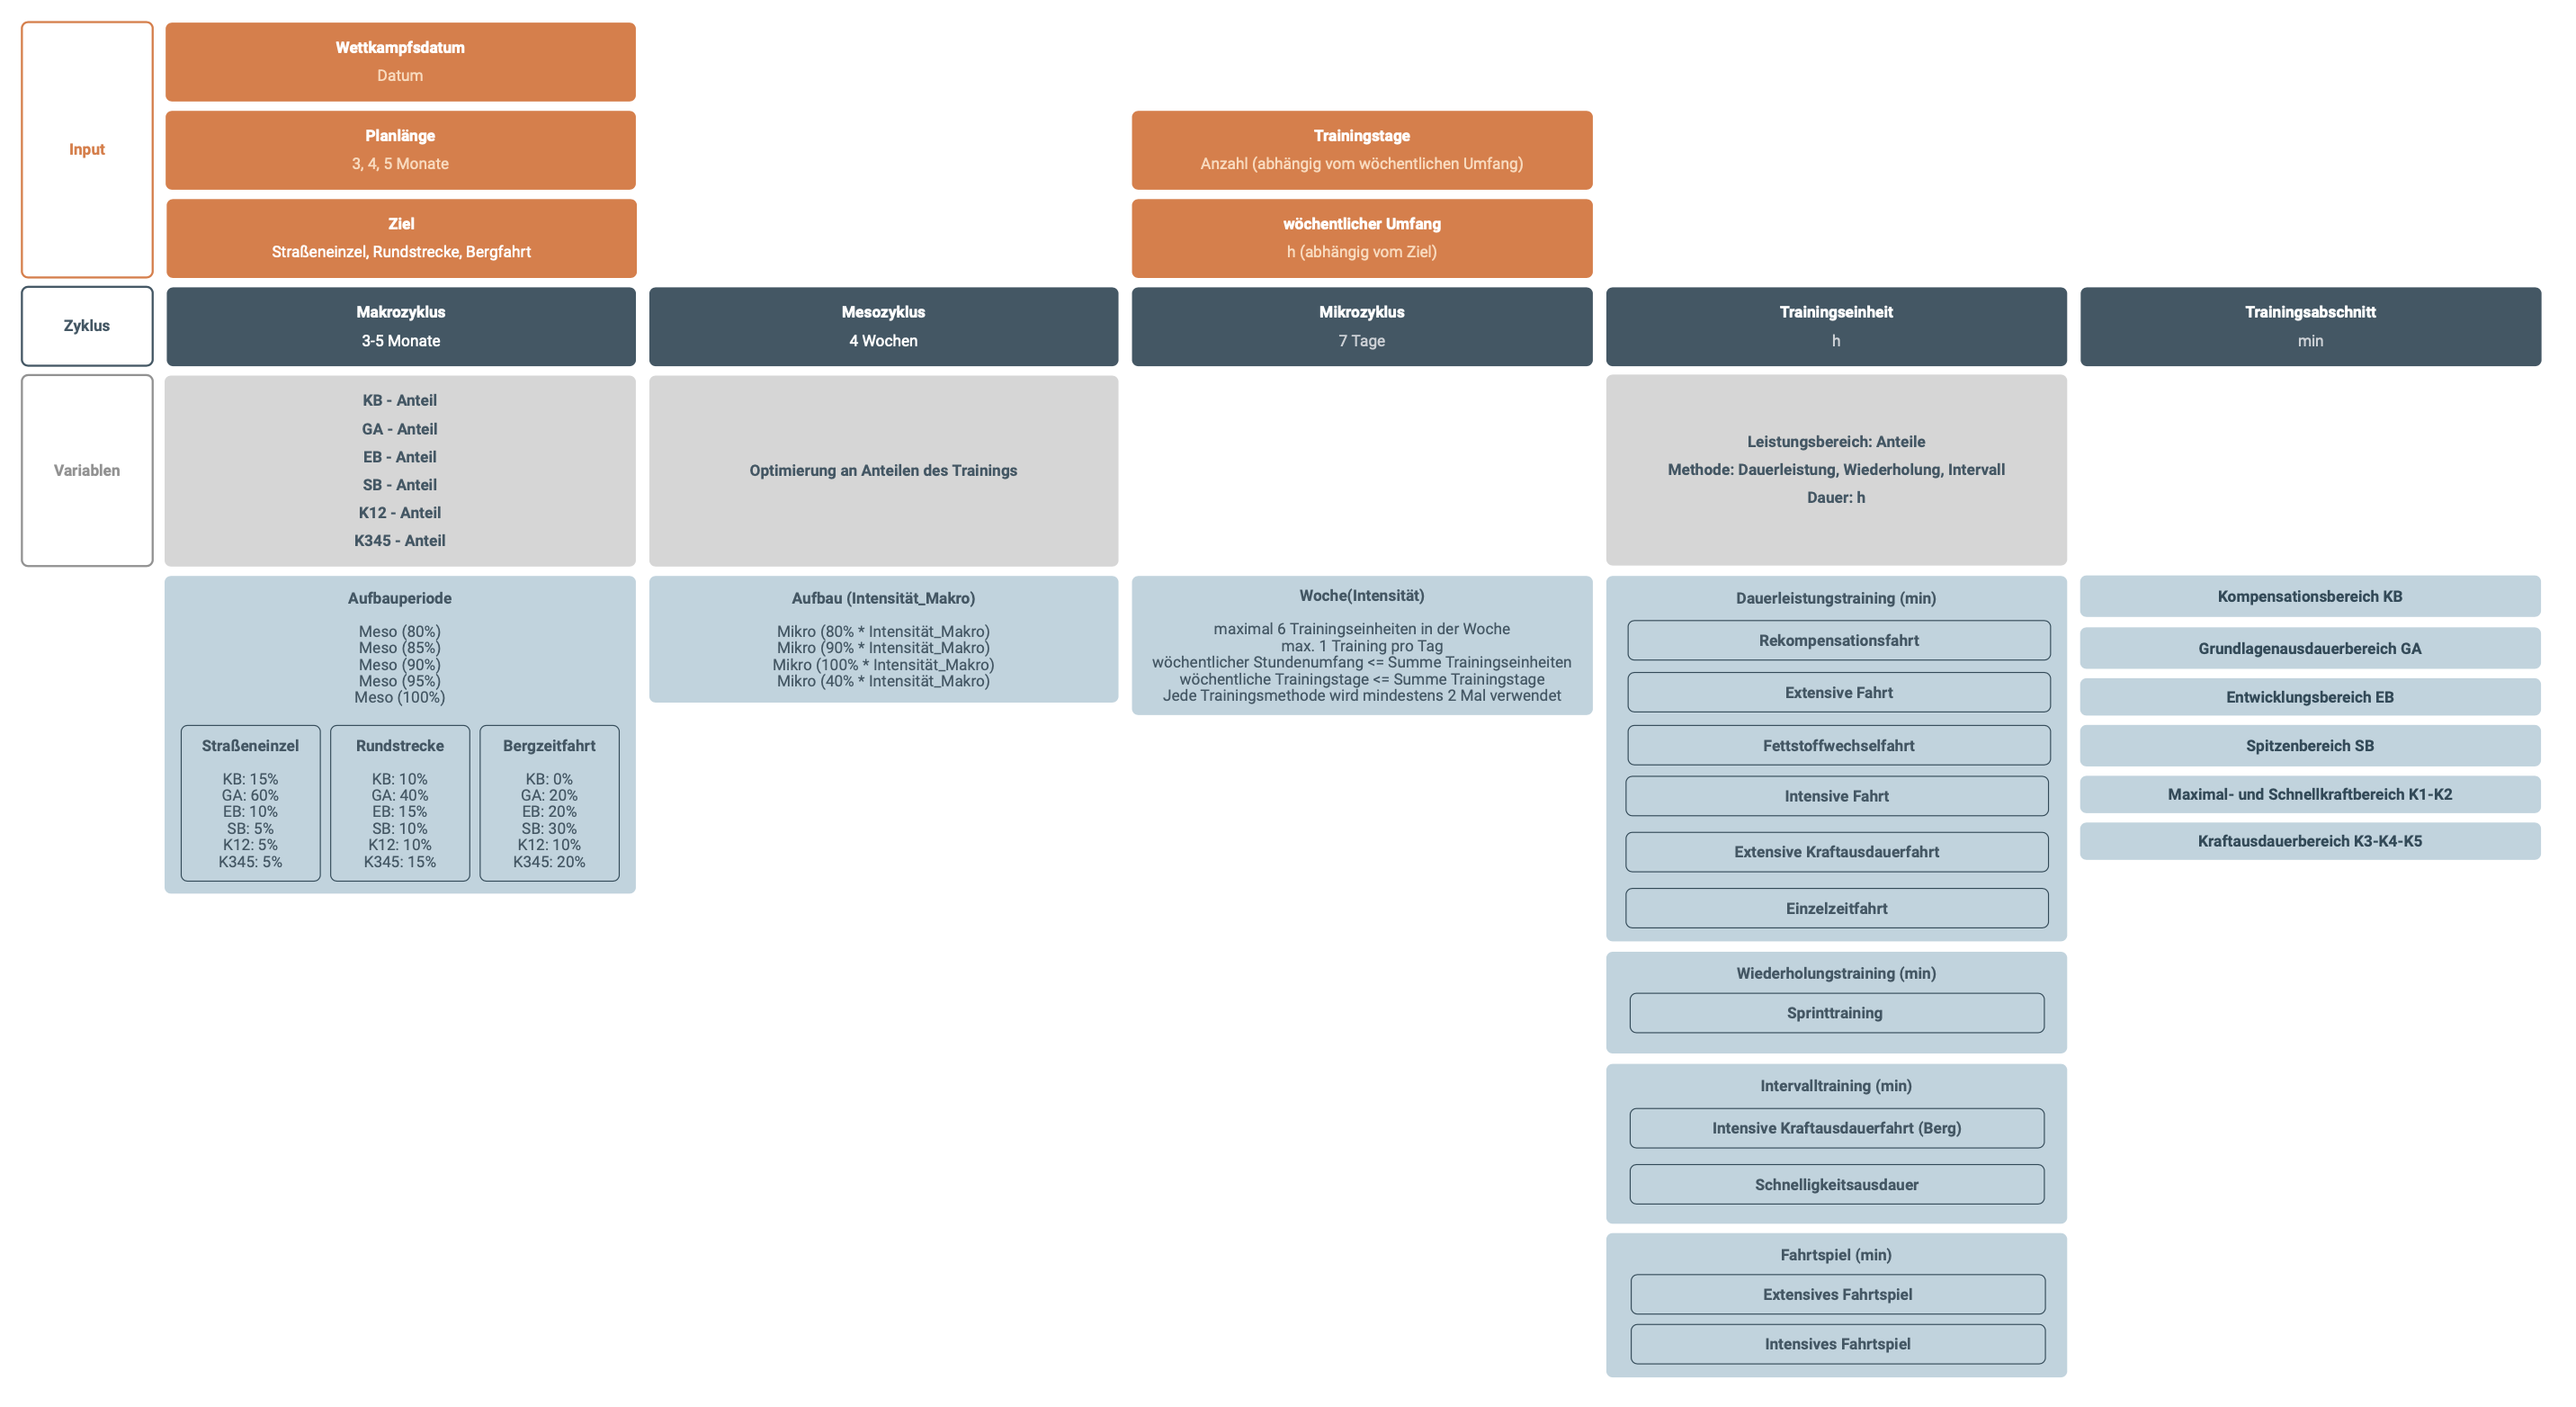
\includegraphics[width=\textwidth]{gfx/modellierung.png}
    	\caption{Schema aus Makro-, Meso- und Mikrozyklen}
    	\label{fig:modellierung:schema}
    \end{figure}
    
Bei der Erstellung eines Trainingsplans wird auf die Constraint Programmierung zurückgegriffen. Dennoch ist der Solver in ein Programm eingebettet, dass bereits die Eingabe und Ausgabe des Benutzers handhabt. Die Validierung von Eingabe und Ausgabe ist so unabhängig von der Modellierung mit Constraint Programmierung. Die Optimierung ist auf Ebene der Mesozyklen implementiert. So wird jeder Monat unabhängig der anderen modelliert. Gesteuert wird die Gewichtung der Leistungsbereiche in den einzelnen Monaten durch zwei Faktoren. Die Länge des Plans (3, 4 oder 5 Monate) bestimmt die Anzahl der Mesozyklen. Desweiteren steigt bei Mesozyklen die Gewichtung der wettkampfsspezifische Ausdauer proportional \TODO{Ist das so?} zur Nähe am Wettkampfstermin.
    \begin{enumerate}
        \item Trainingsziel bestimmen
        \item Einfach-Periodisierung des Trainingplans zum Wettkampfstermin
        \item Vierfach-Periodisierung der Aufbauphase aus Vorbereitungsperioden
        \item Constraints auf Ebene der Hierarchie definieren 
        \item Solver erstellt Trainingseinheiten
    \end{enumerate}
    \subsection{hierarchische Zyklisierung}

\section{Designentscheidungen}
\subsection{Kraftbereiche vs. Trainingsmethoden mit Belastungsstufen einer Einheit}
\subsection{Optimierung auf Ebene der Mesozyklen}
    
\section{Model}
\subsection{Konstanten}
In der Modellierung betrachten wir Konstanten gesondert. Diese Größen sind in jeder Lösungsinstanz relevant aber vor der Modellierung festbestimmt. Weitestgehend entsprechen sie den Eingaben des Benutzers.
Input wöchentlicher Trainingsumfang (Stunden)
$max_{hours} \in [0, 40]$

Input Anzahl wöchentlicher Trainingstage
$max_{days} \in [1, 7]$

Input Trainingsziel
$kb \in [0, 100]$
$ga \in [0, 100]$        
$eb\in [0, 100]$
$sb\in [0, 100]$
$k123\in [0, 100]$
$k45\in [0, 100]$
        
Input Wettkampfstag -> Trainingslänge = Anzahl der Tage
$length \in \{ 84, 112, 140\} $ 
        
\subsection{Variablen}
Unter den Variablen der Modellierung versteht man die veränderlichen Größen.

        
        Variable um den Tag der Trainingseinheit $i$ zu identifizieren
        \begin{equation}
            \forall i \in [1, \text{length}], \text{day}_i = [\![1, \text{length}]\!]
        \end{equation}
    
        Variable um Leistungsbereich der Trainingseinheit $i$ zu identifizieren
        \begin{equation}
            \forall i \in [1, \text{length}], \text{range}_i = [\![0, 6]\!] \text{oder} \{\text{KB, GA, EB, SB, K12, K345}\}
        \end{equation}
        
        Variable um Dauer der Trainingseinheit $i$ zu identifizieren
        \begin{equation}
            \forall i \in [1, \text{length}], \text{duration}_i = [\![0, 10]\!]
        \end{equation}
        
        Variable um Trainingsmethode der Trainingseinheit i zu identifizieren
        \begin{equation}
            \forall i \in [1, \text{length}], \text{method}_i = \{\text{DL, IV, WH}\}
        \end{equation}

    \subsection{Constraints}
    \subsubsection{Allgemein}
    Nur ein Training pro Tag
        \begin{equation}
            \forall i, j \in [1, 150]^2, i\neq j \Rightarrow day_i \neq day_j
        \end{equation}
    Summe der Trainingsstunden unter wöchentlichem Umfang
    \TODO{Definition einer einzelnen Woche}
        \begin{equation}
            \forall i = k * 7 + 1, k \in \math{Z}, \sum_{i}^{i+6} \text{duration}_i \leq max_{hours}
        \end{equation}
        \begin{equation}
            \forall i \in \{ i = k * 7 + 1, k \in \math{Z} \}, \sum_{i}^{i+6} \text{duration}_i \leq max_{hours}
        \end{equation}
    Summe der Trainingstage unter wöchentlichem Maximalwert
        \begin{equation}
            \forall i = k * 7 + 1, k \in \math{Z}, \sum_{i}^{i+6} \text{day}_i \leq max_{days}
        \end{equation}
    Maximal 6 Trainingseinheiten in der Woche
        \begin{equation}
            max_{days} \leq 6
        \end{equation}
    3 Tage vor Wettkampf kein Training (Superkompensation)
    \TODO{duration = 0 oder kein Training?}
        \begin{equation}
            \forall i \in [\text{length}-3, \text{length}] \in \math{Z}, \sum_{i}^{i+6} \text{day}_i \leq max_{days}
        \end{equation}

    \subsubsection{Trainingseinheit}
    KB Einheit hat maximale Dauer von zwei Stunden
        \begin{equation}
            \forall i \in \{i | \text{range}_i = \text{KB}\}, \text{duration}_i \leq 2
        \end{equation}
    KB Einheit immer als Dauerleistungsmethode
        \begin{equation}
            \forall i \in \{i | \text{range}_i = \text{KB}\}, \text{method}_i = \text{DL}
        \end{equation}
    GA Einheit hat Mindestdauer von 1 Stunde
        \begin{equation}
            \forall i \in \{i | \text{range}_i = \text{GA}\}, 1 \leq \text{duration}_i
        \end{equation}
    GA Einheit hat maximale Dauer von fünf Stunden
        \begin{equation}
            \forall i \in \{i | \text{range}_i = \text{GA}\}, \text{duration}_i \leq 5
        \end{equation}
    GA Einheit immer als Dauerleistungsmethode
        \begin{equation}
            \forall i \in \{i | \text{range}_i = \text{GA}\}, \text{method}_i = \text{DL}
        \end{equation}
    SB Einheit immer als Intervallmethode
        \begin{equation}
            \forall i \in \{i | \text{range}_i = \text{SB}\}, \text{method}_i = \text{IV}
        \end{equation}
        
    \subsubsection{Optimierung}
    OPT an Anteilen des Trainings 
        \begin{equation}
            \forall i \in \{i | \text{range}_i = \text{KB}\}, \text{method}_i = \text{DL}
        \end{equation}
        Für die 
        \begin{equation}
            \text{minimiere} \sum_{i=0}^{\text{length}} \text{duration}_i
        \end{equation}
\chapter{Design der Software}
\label{sec:design}

\section{UML Diagramm des Modells}
\label{sec:design:UML}
\begin{figure}[htb]
	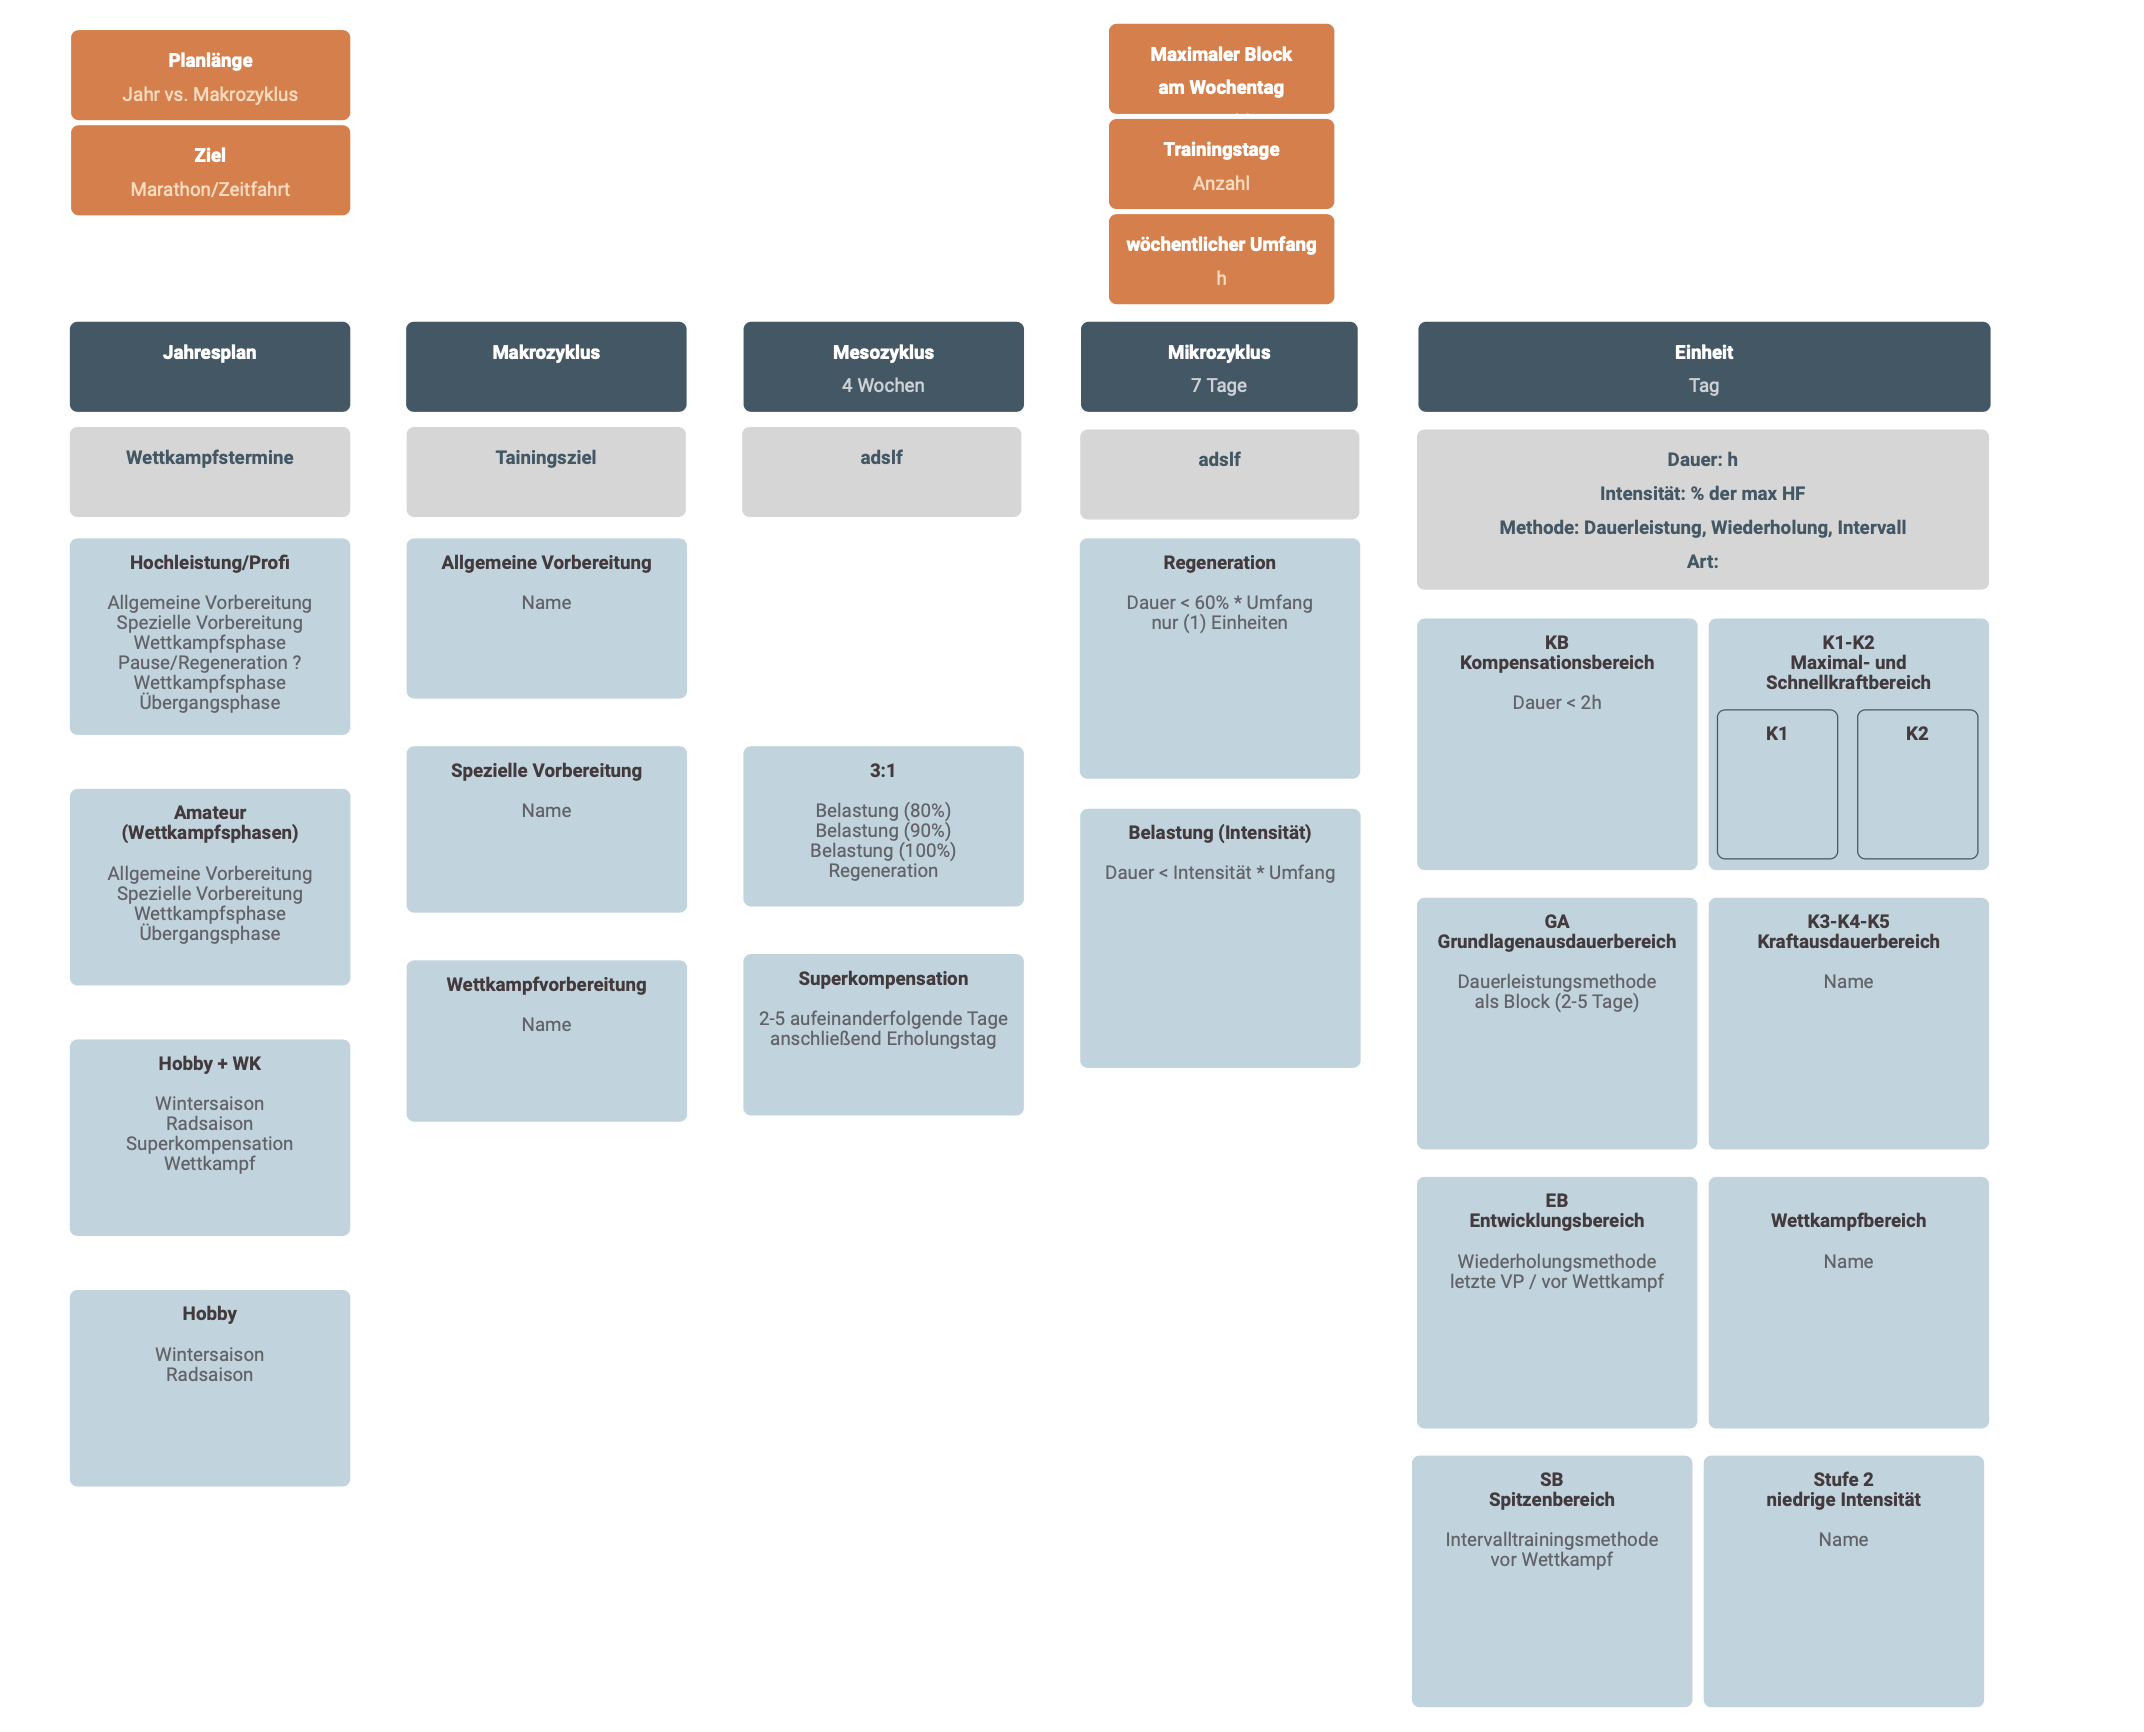
\includegraphics[width=\textwidth]{gfx/uml.png}
	\caption{UML Diagramm}
	\label{fig:system:example1}
\end{figure}
Objektorientiert nach hierarchischer Struktur der Zyklen
\subsection{Trainingseinheit}
    Siehe Kapitel \ref{sec:modellierung}
\subsection{Trainingsplan}
    Als Liste von Trainingseinheiten oder Zyklische Struktur übernehmen
 
\section{Template Design Pattern}
\label{sec:design:template}
Template Method um verschiedene Zielgruppen umzusetzen

Profi (Trainingsumfang > 20h)

Amateur (Trainingsumfang < 20h)

Hobbyfahrer (Trainingsumfang < 4h)

\chapter{Implementierung}
\label{sec:implementierung} 
Bei der Implementierung der Modellierung wird die objektorientierte Programmiersprache JAVA \cite{java} verwendet. Nativ bietet sie keine Constraint Programmierung an, aber diesbezüglich wird auf choco-solver \cite{ChocoSolverWeb} zurückgegriffen. Mit dieser Open-Source Bibliothek ist die Modellierung von persönlichen und Lehrprojekten möglich. \par
Aus der Hierarchie der Zyklen lassen sich die Objektklassen entwerfen. Auch wenn die übergeordnete Instanz der Makrozyklus ist, erfolgt die Optimierung erst auf Ebene des Mesozyklus \hyperref[sec:modellierung:model]{(siehe Kapitel \ref{sec:modellierung:model})}. So wird jeder Monat unabhängig der Anderen modelliert und der Einsatz des choco-solvers auf die \texttt{Meso}-Klasse beschränkt. Gesteuert wird die Gewichtung der Leistungsbereiche in den einzelnen Monaten durch zwei Faktoren. Die Länge des Plans (3, 4 oder 5 Monate) bestimmt die Anzahl der Meso-Instanzen im Makrozyklus. Des Weiteren steigt bei Mesozyklen die Gewichtung der wettkampfsspezifischen Ausdauer bei Näherung an den Wettkampfstermin.
Dennoch ist der Solver in ein Programm eingebettet, dass bereits die Eingabe und Ausgabe des Benutzers handhabt. Die Interaktion mit dem Programm ist so unabhängig von der Modellierung. \par

\section{Eingaben}
Um den Trainingsplan zu individualisieren erfasst das Programm die Eingaben des Nutzers. Die Wettkampfsdisziplin korreliert mit dem Trainingsziel. An der ausgewählten Disziplin macht sich dann die Gewichtung der Leistungsbereiche fest. Der wöchentliche Trainingsumfang des Plans limitiert die Trainingszeit pro Woche. Die Anzahl der Stunden lässt auch Rückschlüsse auf die Professionalität zu. Während im Profibereich der Trainingsumfang über 20 Stunden beträgt, unterschreiten Amateure diesen Wert üblicherweise. Bei einem Wert bis zu 5 Stunden, spricht man oft von Freizeitsport. \TODO{Belegen} \newline
Nicht nur die wöchentlichen Stunden, sondern auch die wöchentlichen Trainingstage werden bei der Erstellung des Plans berücksichtigt. Die Anzahl der Tage steuert die Häufigkeit der Einheiten.
Wie in \ref{grundlagen:sport:belastungsbereiche} aufgeführt, umfasst ein Training mehrere Belastungsbereiche. Weitestgehend werden die Konstanten der Modellierung über die Eingabe erfasst. 
\begin{itemize}
    \item Ziel/Disziplin: Straßeneinzelrennen, Rundstrecke, Bergzeitfahrt
    \item wöchentlicher Trainingsumfang: Anzahl Stunden
    \item wöchentliche Trainingstage: Anzahl Tage
    \item Wettkampfstermin: Datum
    \item Dauer des Plans: 3/4/5 Monate
\end{itemize}

\section{UML-Diagramm der Modellierung}
\begin{figure}[h]
    \begin{tikzpicture}
        \umlclass[y=5, fill=white, type = abstract]{Macro}{
            - sessions : ArrayList<Session> \\
            - numMonth : int \\
            - maxTrainingMinutes : int \\
            - maxTrainingDays : int \\
            - compDay : Date \\
            - ranges : HashMap<Range, Double> \\
        }{
            + solvePlan() : void \\
            \textit{+ setRanges() : void} \\
            + validateRanges() : void \\
        }
        
        \umlclass[x=8, y=5, fill=white]{Meso}{
            - model : Model \\
            - plan : Solution \\
            - startDay : Date \\
            - targetRanges : int[6] \\
            - targetMinutes : int[4] \\
            - name : IntVar[] \\
            - minutes : IntVar[] \\
            - method : IntVar[] \\
            - ranges : IntVar[][] \\    
            - distanceRanges : IntVar[] \\
            - overallDistance : IntVar \\

        }{
            - initializeModel() : void \\
            - defineConstraints() : void \\
            + solveMonth() : void \\
            + getPlan() : Solution \\
        }
        \umlclass[x=8, y=-3, fill=white]{Session}{
            - name : String \\
            - minutes : int \\
            - distribution : HashMap<Range, Integer> \\
            - day : LocalDate \\
            - method : Method \\
        }{}
        \umlclass[x=1, y=0, fill=white]{Strasseneinzel}{}{+ setRanges() : void}
        \umlclass[x=1, y=-2, fill=white]{Rundfahrt}{}{+ setRanges() : void}
        \umlclass[x=1, y=-4, fill=white]{Bergfahrt}{}{+ setRanges() : void}
        
        \umlHVinherit[anchor2=-130]{Strasseneinzel}{Macro}
        \umlHVinherit[anchor2=-130]{Rundfahrt}{Macro}
        \umlHVinherit[anchor2=-130]{Bergfahrt}{Macro}
        \umluniassoc[arg=-mesos ,  mult2=3..5, pos =0.95, align=right]{Macro}{Meso}
        \umluniassoc[arg=-sessions , mult2=28, pos =0.80, align=right]{Meso}{Session}
    \end{tikzpicture}
    \caption{UML Diagram der Modellierung}
    \label{fig:uml:solver}
\end{figure}

\subsection{Macro-Klasse}
Diese Klasse koordiniert das Erstellen der Mesozyklen und ist der Einstiegspunkt für Operationen auf den Trainingsplan. Je nach Planlänge, wird für jeden Monat eine Mesoinstanz generiert. Hierfür werden aus dem Prinzip der Periodiesierung und progressiven Belastung bereits die Zielwerte in den einzelnen Wochen berechnet, um sie an die Mesozyklen weiterzugeben.
Die Lösungsinstanzen der Mesozyklen ergeben dann zusammengesetzt den Trainingsplan. Das ist analog zur Hierarchie der Zyklen gestaltet. \newline
Über Vererbung werden die verschiedenen Wettkampfsdisziplinen realisiert. Die Hook-Operation \texttt{setRanges()} definiert für jeden Belastungsbereich die Gewichtung. Mit \texttt{validateRanges()} wird sichergestellt, dass diese Verteilung zu 1 summiert. 
Um Laufzeit zu optimieren wird die Optimierung der einzelnen Mesoinstanzen parallelisiert angestoßen.

\subsection{Meso-Klasse}
Gekapselt in eine Klasse wird hier die Modellierung von 28 Tagen vorgenommen. Zum Einsatz kommt hier der choko-solver. Für die Variablen werden die zugehörigen IntVar-Klassen angelegt. \TODO{Hier den Code einfügen?} 
Nach dem Lösungsprozess erstellt die Klasse aus den Werten die passenden Sessionobjekte für jeden der 28 Tage.
Um die Modellierung in angemessener Zeit zu ermöglichen wurde mithilfe des choko-Solvers eine zeitliche Begrenzung von 30 Sekunden für den Löäsungsprozess festgelegt. So kann der Lösungsprozess besser gesteuert werden. Durch die Diskretisierung der Belastungsbereiche ist die exakte Vorgabe an Minuten eventuell gar nicht zu treffen. Die genauer Evaluation der erstellten Trainingspläne erfolgt in \hyperref[sec:evaluation]{Kapitel \ref{sec:evaluation}}.

\subsection{Session-Klasse}
Die Sessionobjekte vereinfachen die Visualisierung. Die enthalten alle charakteristischen Daten eines Trainingstages auf die in \ref{sec:modellierung:output} eingegangen wird/wurde. 

\section{Modularisierung}
Die Grundlage dieser Arbeit war eine vorangegangene Bachelorarbeit, die der Laufsport betrifft. Mit Ausblick auf die Erweiterung um das Schwimmtraining, ist durch Kombination dieser Arbeiten vorstellbar zu einem Trainingsplan für Triathleten. 
Aus diesem Grund ist die Arbeit modular gegliedert.
Für viele Sportarten gelten die Trainingsprinzipien der Zyklisierung, Periodisierung, progressive Belastung und Superkompensation. Diese Struktur kann für andere Ausdauersportarten übernommen werden. Um die Trainingsplanerstellung für andere Sportarten zu modellieren, sind folgende Erweiterungen im Code nötig. \par
Die Definition der Leistungsbereiche, Trainingsmethoden und validen Trainingseinheiten ist über Aufzählungstypen (engl. enumeration) erfolgt. Diese enthalten spiegeln eine endliche Wertemenge wieder.\par
\begin{figure}[h]
    \centering
    \begin{tikzpicture}
        \umlclass[type=enumeration, fill=white]{Range}{
            Kompensation   \\ 
            Grundlagenausdauer   \\ 
            Entwicklungsbereich   \\ 
            Spitzenbereich   \\ 
            Kraftausdauer1   \\ 
            Kraftausdauer4   
        }{}
        
        \umlclass[type=enumeration, x=4.25, fill=white]{Method}{
            Pause \\
            Dauerleistung   \\ 
            Fahrtspiel  \\
            Intervall \\
            Wiederholung  \\
        }{}
        \umlclass[type=enumeration, x=9, fill=white]{SessionPool}{
            Pause\\
            Kompensationstraining \\
            ExtensiveFahrt   \\ 
            Fettstoffwechsel  \\
            IntensiveFahrt \\
            ExtensiveKraftausdauerfahrt  \\
            Einzelzeitfahrt  \\
            ExtensivesFahrtspiel  \\
            IntensivesFahrtspiel  \\
            IntensiveKraftausdauer  \\
            Schnelligkeitsausdauer  \\
            Sprinttraining  \\
        }{
            getPause() \\
            getDL() \\
            getFS() \\
            getIV() \\
            getWH() \\
        }
    \end{tikzpicture}    
    \caption{Enumeration um sportartspezifisches zu Kapseln}
    \label{fig:uml:enumeration}
\end{figure}
Die Erweiterung des Modells um weitere Leistungsbereiche in Range ist möglich, aber erfordert im SessionPool die Festlegung der Zeitspannen für diesen Belastungsbereich. Eher ist davon auszugehen, dass nach der Festlegung für eine Sportart die Belastungsbereiche final sind. Vorteil der Kapselung ist hier, dass eine neue Kombination dieser drei Aufzählungstypen genutzt werden kann um mit dem Modell andere Ausdauersportarten zu lösen. Denn die konkreten Belastungsbereiche beeinflussen die Modellierung nicht. Diese ist unabhängig von sportartspezifischen Ausprägung der Trainingseinheiten implementiert. Die Liste der Trainingsmethoden dient zur Zuweisung der Trainingseinheiten zu ihrer Trainingsmethode. Im SessionPool sind die Trainingseinheiten definiert mit ihren möglichen Zeitspannen je Belastungsbereich. Neue Arten von Trainingseinheiten können also mit geringem Aufwand hinzugefügt werden. Das Ändern der Modellierungsklasse ist dafür nicht erforderlich.

\section{Ausgabe}
\label{sec:modellierung:output}
Die Ausgabe des Plans ist über zwei Wege verfügbar. In der Implementierung ist eine grafische Benutzungsoberfläche zur tabellarischen Ansicht der Trainingseinheiten inklusive. Über die grafische Schnittstelle erfolgen die Eingaben und nach Erstellung des Plans auch die Möglichkeit diesen als PDF-Dokument abzuspeichern. Die Trainingseinheit wird definiert durch die nachfolgenden Parameter.
\begin{figure}[h]
    \begin{tikzpicture}
        \umlclass[y=5, fill=white]{Main}{
            - plan : Macro
        }{
            + monitorStats() : void \\
            + createPlan() : void \\
            + createTable(i : int) : void \\
            + createPDF(i : int) : void \\}
        \umlclass[x=9, y=5, fill=white]{OutputTrainingTable}{
        }{
            + displayPlan() : void \\
        }
        \umlVHVassoc[]{Main}{OutputTrainingTable}
    \end{tikzpicture}    
    \caption{UML-Diagram für die Interaktion mit dem Modell}
    \label{fig:uml:solver}
\end{figure}
\begin{itemize}
    \item Tag: Datum
    \item Dauer: Anzahl Stunden
    \item Trainingsarten: TrainingPool \ref{anhang:trainingsarten}
    \item Trainingsbereich: Range \ref{grundlagen:sport:belastungsbereiche}
    \item Trainingsmethode: Method \ref{grundlagen:methoden}
\end{itemize}

Das UML-Diagramm des vollständigen Programms ist im Anhang unter \ref{anhang:uml} aufgeführt und besteht aus der Zusammensetzung der obigen Teile.

% ALTERNATIVSÄTZE
% Außerdem besteht die Möglichkeit den Trainingsplan als einfaches PDF-Dokument herunterzuladen.
% Darstellung der Trainingseinheiten als Liste in der Java Applikation
% Die konkrete Umsetzung des Softwareprojekts wird als Java-Anwendung zur Verfügung gestellt.
% Alle oben genannten Funktionen werden unterstützt.Bei der Lösung des Optimierungsproblems kommt das Framework choco-solver zum Einsatz. Die Optimierung wird ausgelöst auf jeden Monat.
% Die Berechnung einer Lösunginstanz der Mesozyklen wird parallelisiert ausgeführt.

% Übertragbarkeit auf andere Sportarten? Welche Constraints sind speziell für den Radsport vs. allgemeine Trainingsprinzipien
% modulare Entwicklung der Anwendung?
% Einbettung des Solvers in Java Programm
% Time Limits oder andere Arten zur Steuerung des Solvers -> Kommt dann in Implementierung
% ? Trainingsalternativen = Auswahl an möglichen Einheiten
\chapter{Zusammenfassung}
\label{sec:zusammenfassung}
\section{Ergebnis der Arbeit}
\label{sec:zusammenfassung:ergebnis}
Die Arbeit hat gezeigt, dass die Erstellung eines Trainingsplans durch Constraint Programmierung lösbar ist. Zu diesem Zweck sind die trainingswissenschaftlichen Anforderung an einen Trainingsplan definiert worden. Der Trainingsplan beachtet die Trainingsprinzipien der Zyklisierung, Periodisierung und progressiven Belastung. Er plant die Aufbauphase in Abhängigkeit der angegebenen Wettkampfsdisziplin. Welche Leistungsbereiche des Radsports abgedeckt werden steht damit in einem direkten Zusammenhang.\newline 
Zusammengesetzt wird ein Plan nach dem Baukastenprinzip. Die dynamisch definierten Trainingseinheiten sind Bausteine und haben verschiedene Anteile an den Leistungsbereichen. Das mathematische Modell optimiert die Auswahl der Einheiten, sodass die Anteile der Leistungsbereiche im Plan denen des Trainingsziels entsprechen. Begrenzt wird der wöchentliche Trainingsumfang in Stunden aber auch Tagen. Auch die Variation der Trainingsmethoden nimmt Einfluss auf die Wahl.\newline
Die Modellierung ist in eine eigenständige Anwendung umgesetzt. Die Benutzung erfolgt über eine übersichtliche grafische Benutzeroberfläche. Auf Ebene der Mesozyklen parallelisiert die Software das Lösen der einzelnen Monate. Zusammengesetzt ergeben diese den vollständigen Trainingsplan der Aufbauphase. Durch den modularen Aufbau des Programmcodes bietet die Arbeit eine Grundlage für die Weiterentwicklung. Das Programm listet die Trainingseinheiten nach der Berechnung und ermöglicht sie als PDF-Dokument abzuspeichern.\newline
Anhand zweier beispielhafter Pläne bestätigt sich die Praktikabilität der Anwendung. Die gemessenen Abweichungen in den einzelnen Bereichen sind vertretbar, denn die Diskrepanz zum Zielwert beträgt durchschnittlich \TODO{Prozent} der Trainingsminuten. Die Anwendung terminiert in angemessener Zeit und deckt die Zielgruppe aus Freizeitsportler:innen und Amateursportler:innen erfolgreich ab.
\TODO{Überleitung}

\section{Ausblick}
\label{sec:zusammenfassung:ausblick}
Obwohl die Erstellung eines Trainingsplans erfolgreich umgesetzt wurde, gibt es Möglichkeiten zur Verbesserung und Weiterentwicklung. Auf die verschiedenen Ansätze wird nachfolgend eingegangen.

\subsection{Präzisierung}
In dieser Modellierung geben die wichtigen Grundlagen der Trainingswissenschaft die Bedingungen vor. Dennoch deckt das Modell nicht alle Details ab, die Einfluss auf die Qualität eines Trainingsplans haben. Ein exaktes System ist in der Form zwar durch die Natur der Trainingswissenschaft nicht möglich, dennoch gibt es weitere etablierte Trainingsprinzipien. \par
Durch das Aufnehmen weiterer Abhängigkeiten steigt besonders die Individualität des Plans. Mögliche Größen mit Einfluss auf den Trainingsplan sind zu untersuchen. Darunter fallen Einfluss des Alters bzw. des Trainingsalters \cite[181]{EinfuerungTrainingswissenschaft}, des Geschlechts und die Leistungsgruppe \cite[S. 173]{Radsporttraining}.\par
Darüber hinaus ist sogar ein vorangestellter Leistungstest vorstellbar. Die eine Art der Leistungsdiagnostik ermittelt den Gesundheitsstand. Beispielsweise . Mithilfe dieser Informationen kann bei der Ausgabe der Trainigseinheiten näher auf die Steuerparameter (Herzfrequenz) der Leistungsbereiche eingegangen werden.  Defizite in einzelnen Bereichen können --  wie die Wettkampfsdisziplin -- auf die Anteile der Leistungsbereiche Einfluss nehmen. Das hohe Maß an Individualität, das dadurch gewonnen wird, verlangt jedoch mehr Aufwand v voraus. \par
In der Constraint Programmierung besteht die Möglichkeit Soft-Constraints zu definieren. Deren Erfüllung ist optional und bei einer Lösungsinstanz nicht immer gegeben. Falls die Randbedingung nicht erfüllt ist, wird die Instanz bei der Optimierung aber schlechter bewertet. Der choco-Solver unterstützt diesen Mechanismus nicht direkt. Jedoch erlaubt er über Reified-Constraints den Status der Erfüllbarkeit abzufragen. Addiert man die Anzahl der nicht erfüllten Bedingungen auf den Optimierungswert, rekonstruiert es die gleichen Effekte wie ein Soft-Constraint. Interessant ist das dann bei Empfehlungen der Trainingsplangestaltung. Zum Beispiel rät man zu einem Erholungstag vor Einheiten, die einen großen Anteil an K123- oder K45-Belastungen beinhalten. Auch die Verteilung der Regenerationstage kann damit gleichmäßiger erfolgen. Folgen viele Tage ohne Trainingseinheit aufeinander, wird das schlechtere Werte erhalten, weil regelmäßige Erholung einer Geballten vorzuziehen ist.
   
\subsection{Erweiterung} 
Auf Grundlage dieser Arbeit ist es möglich die Trainingsplanerstellung weiterzuentwickeln. 
Aus der hierarchischen Struktur folgt die Modularisierung des Programms in Objektklassen.
Denkbar sind andere Ausdauersportarten und die Ausweitung der Trainingsziele. 
Des Weiteren ist die Erweiterung der Makrozyklen auf die Vorbereitungsperiode und Übergangsperiode möglich. So wären die Bausteine für einen Jahresplan vorbereitet. \\ \\
Anderweitige Belastungen, ungeplante Ausfälle
Wie wirkt sich Training außerhalb des Radsports aus? z.B. Ein Fußballer, der auch Rennrad fährt. \\ \\
Triathleten und andere Sportarten
Zusammenschluss der Arbeiten dann zu einem Trainingsplan spezifisch für die Triathlon Vorbereitung möglich? \\ \\
Trainingsdokumentation
Erweiterung zur Trainingskontrolle und Trainingsdokumentation

\subsection{Performance}
eigene Suchstrategie für Laufzeitoptimierung
Diese Arbeit benötigt für die Erstellung des Plans maximal 30 Sekunden. Dieses Limit wurde der Modellierung hinzugefügt, um ein anwendbares System zu erhalten. Durch die zeitliche Begrenzung des Lösungsprozesses, toleriert die Lösung auch eine Abweichung von den Leistungsbereichen. Die Optimierung wird vorgenommen, es ist jedoch nicht garantiert, dass die vorgegebene Lösung optimal (Distanz = 0) ist. Grund dafür ist die Diskretisierung der Leistungsbereichanteile auf fünf Minuten und die der Trainingseinheiten auf viertelstündliche Vorgaben, aber auch das Limitieren des Suchprozesses auf \TODO{Sekunden} Sekunden. Diese beiden 

Verbessert man die Laufzeit der Lösungssuche durch eine bessere Suchstrategie, verringert das auch die Distanz der Leistungsbereiche zur Zielverteilung. Die Lösung nach \TODO{Timerzeit} Sekunden ist näher am optimalen Wert.

\subsection{Zugänglichkeit}
Fokus dieser Arbeit war die Modellierung eines optimierten Trainingsplans, weshalb sie als eigenständige Anwendung umgesetzt ist. Um das System der Zielgruppe zur Verfügung zu stellen ist eine Webanwendung zweckmäßiger. 
Durch die Definition einer Schnittstelle mithilfe von JSON-Objekten kapselt sich die Modellierung von der Benutzerinteraktion ab. Nötig ist hierfür das Deployment der Anwendung auf einem JAVA Server. Nachfolgend eine Möglichkeit für eine Schnittstelle.
\begin{minipage}{\linewidth}
\begin{lstlisting}
{ 
    "num_months": 3,
    "competition": "singleday",
    "sport": "racing bike",
    "competition_date": 22.02.2022,
    "sessions": [
        {
            date: 01.02.2022,
            minutes: 60,
            method: "intervall",
            name: "sprinttraining", 
            sections: [
                {
                    length: 45,
                    range: "GA"
                },
                {
                    length: 5,
                    range: "EB"
                },
                ...
            ]
        }
    ], 
}
\end{lstlisting}
\end{minipage}
Die grafische Oberfläche bessere Beschreibung der Trainingseinheiten erweitert werden. 
Mit einer Schnittstelle zur Trainingsplanerstellung Oberfläche/Ausgabe auch maximale Stunden für jeden Wochentag: h/Tag
Oberfläche/Ausgabe auch Trainingseinheit benennen.

% \subsection{Einfluss des Wettkampfdatums}
% Aktuell ist der Starttag immer auf einen Montag festgelegt. Auch wenn 
% Wie die optimale Leistungsbelastung bestimmen ohne Leistungsmesser? Ist das überhaupt nötig, wenn keine Trainingskontrolle stattfinden soll? Test um Leistungsstand zu ermitteln?
%Intensität in einer Trainingseinheit variieren? Angaben zur Intensitätsstufe/min -> ein Pool von möglichen Trainings empfehlen -> auch nicht, sondern Trainingsabschnitte nach Trainingsmethoden definieren
%\item Übertraining verhindern durch Regenerationssteuerung. Es werden keine Messungen/Anpassung im Trainingsverlauf vorgenommen, sodass Übertrainingszustände durch Einplanen von ausreichenden Regenerationsphasen verhindert werden sollen.
%Leistungsnachlass durch zu lange Pausen/Regenerationsphasen verhindern (weniger als 5 Tage und 10 Tage)
%\item \TODO{Progression an Trainingsminuten eigentlich ja nicht Belastung dann oder? Also Intensität wäre nötig!}
%\end{itemize}
%\begin{itemize}
%    \item nur x aufeinanderfolgende Tage
%    \item GA Trainings am Besten als Block \cite[34]{Radsporttraining}
%\end{itemize}
\cleardoublepage

% --------------------------
% Back matter
% --------------------------
{%
\setstretch{1.1}
\renewcommand{\bibfont}{\normalfont\small}
\setlength{\biblabelsep}{0pt}
\setlength{\bibitemsep}{0.5\baselineskip plus 0.5\baselineskip}
\printbibliography[nottype=online]
\printbibliography[heading=subbibliography,title={Webseiten},type=online,prefixnumbers={@}]
}

\cleardoublepage
\listoffigures

\cleardoublepage
\listoftables

\cleardoublepage
\pagestyle{empty}
\hfill
\vfill
\pdfbookmark[0]{Colophon}{Colophon}
\section*{Colophon}

Diese Bachelorarbeit wurde gesetzt mit \LaTeXe. Sie verwendet den \textit{Clean Thesis} stil entwickelt on Ricardo Langner. Das Design ist inspiriert vom Benutzerhandbuch von Apple Inc.

Der \textit{Clean Thesis} Stil ist verfügbar unter \url{http://cleanthesis.der-ric.de/}.

%This thesis was typeset with \LaTeXe.
%It uses the \textit{Clean Thesis} style developed by Ricardo Langner.
%The design of the \textit{Clean Thesis} style is inspired by user guide documents from %Apple Inc.

%Download the \textit{Clean Thesis} style at \url{http://cleanthesis.der-ric.de/}.

\cleardoublepage
\pdfbookmark[0]{Declaration}{Declaration}
\chapter*{Erklärung}
\label{sec:declaration}
\thispagestyle{empty}

Hiermit versichere ich, dass ich die vorliegende Arbeit selbstständig und ohne Benutzung anderer als der angegebenen Hilfsmittel angefertigt habe. Die aus anderen Quellen oder indirekt übernommenen Daten und Konzepte sind unter Angabe der Quelle gekennzeichnet. Die Arbeit wurde bisher weder im In- noch Ausland in gleicher oder ähnlicher Form in einem Verfahren zur Erlangung eines akademischen Grades vorgelegt.

\bigskip

\noindent\textit{\thesisUniversityCity, \thesisDate}

\smallskip

\begin{flushright}
	\begin{minipage}{5cm}
		\rule{\textwidth}{1pt}
		\centering\thesisName
	\end{minipage}
\end{flushright}

%*****************************************
%*****************************************

\clearpage

\newpage
\mbox{}
\end{document}
